\chapter{Materiais e Métodos}


A metodologia proposta neste trabalho visa a aplicação de técnicas de quantificação
de risco de um projeto hipotético de poço petrolífero na fase de perfuração. As abordagens propostas para quantificação de risco consistem na utilização das metodologias da Árvore de derivação e de Monte Carlo, que por sua vez, estão subsidiadas pela aplicação de Planejamento estatístico para geração de metamodelos (\textit{Proxy models} ou \textit{Surrogate models}), que possam substituir o simulador fluidodinâmico na quantificação do desgaste erosivo em cenários que demandam muitas simulações.
A metodologia de análise de risco é focada na geração de diversos cenários possíveis de fluxo, compostos pela combinação dos atributos incertos que influenciam na resposta de desgaste erosivo através dos métodos de Árvore de Derivação (AD) e Monte Carlo (MC). As principais etapas desta metodologia são:

\begin{itemize}
  \item Escolha dos atributos incertos que influenciam no desgaste erosivo segundo estudo bibliográfico;
  \item Definição das distribuições de probabilidades das variáveis aleatórias e probabilidades de ocorrência associadas a cada nível discretizado;
  \item Triagem e seleção dos atributos críticos, ou seja, que exercem maior impacto no desgaste erosivo, através da Análise de sensibilidade e Planejamento Plackett Burmann;
  \item Geração de metamodelo através de Planejamento estatístico Box Behnkhen para previsão do desgaste erosivo em substituição ao simulador numérico;
  \item Geração de cenários de simulação através da combinação dos atributos críticos através das técnicas de Àrvore de derivação Monte Carlo;
  \item Obtenção da curva de risco das funções-objetivo através do tratamento estatístico e
obtenção dos percentis P10, P50 e P90. 
\end{itemize}

\section{Variáveis aleatórias e distribuições de probabilidades}
\label{cap:Variáveis aleatórias e distribuições de probabilidades}

 Para obter a análise de risco de um projeto, são necessárias amostragens das variáveis aleatórias que influenciam no fenômeno estudado. Os atributos que influenciam no desgaste erosivo, segundo a literatura, foram expostos no capítulo \ref{cap:Erosão por partículas sólidas}. Para esta dissertação, as variáveis aleatórias consideradas para as previsões de desgaste erosivo foram: Tamanho do cascalho, Forma do cascalho, Densidade do cascalho, Densidade do fluido de perfuração, Viscosidade do fluido de perfuração, Velocidade de escoamento e Vazão mássica (Figura \ref{fig:erosaoatb2}). 

\begin{figure}[H] 
    \centering  
    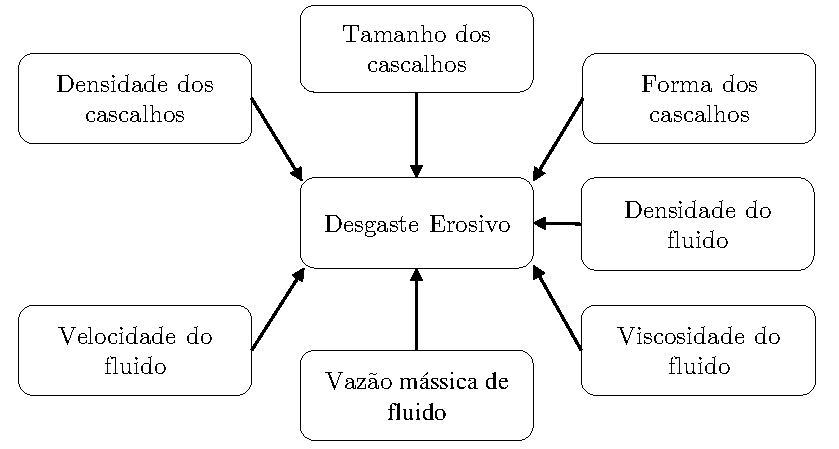
\includegraphics{Figuras/erosaoatb2.pdf}  
    \caption{Relação das variáveis aleatórias consideradas para análise de risco de falha.}  
    \legend{Fonte: o autor.}
    \label{fig:erosaoatb2}  
\end{figure}

As variáveis relativas à propriedade do material alvo não foram consideradas variáveis aleatórias neste estudo (Dureza, Microestrutura) pois apenas a curva de Aço Carbono de 90º e suas propriedades são consideradas na análise de desgaste erosivo. 

A aquisição de dados e amostragens de perfuração é muito dificultosa, uma vez que a maioria das informações obtidas pelas operadora petrolíferas, geralmente, são tratadas com sigilo. Além disso, a obtenção de algumas informações demandam altos investimentos e tempo para serem coletadas. De posse de dados reais, são realizados testes de aderência para caracterizar a distribuição de frequência das variáveis segundo testes estatísticos. Portanto, diante do exposto, para aplicação da metodologia de análise de risco, os dados utilizados nesta dissertação são sintéticos e fictícios, ou seja, as distribuições das variáveis aleatórias foram elaboradas para este estudo de caso hipotético. Os intervalos das distribuições contínuas geradas para o trabalho foram baseadas em valores mínimos, médios e máximos de acordo com a literatura \cite{bortotti} \cite{santoss2} \cite{pereira}, através destes valores foram geradas distribuições de probabilidades (gamma, normal, lognormal e triangular) para representação amostral das variáveis aleatórias. 

Após definição das distribuições de probabilidade, foram discretizados os níveis de incerteza, os valores de cada atributo e as probabilidades de ocorrência associada a cada nível, relacionados na Tabela \ref{tab:atributos}. Foi admitida total independência entre os atributos, ou seja, todas as combinações de atributos na construção de um modelo de fluxo multifásico para análise de erosão são possíveis.

 Os atributos incertos foram discretizados em três níveis de acordo com as respectivas distribuições de probabilidade geradas, com intuito de realizar as metodologias de análise de risco por Árvore de derivação, os planejamentos estatísticos subsequentes, para determinação do impacto dos atributos na taxa erosiva e para criação do metamodelo de regressão através da metodologia de Superfície de resposta. O nível "0" representa o valor mais provável do atributo, o nível "–1" configura o nível inferior e o nível "1" descreve o nível superior da discretização de cada variável aleatória. A Figura \ref{fig:discretizacao} demonstra, como exemplo, a função de distribuição de probabilidade da variável de "Forma dos cascalhos" e sua discretização em diferentes níveis com probabilidades associadas.

\begin{figure}[H] 
    \centering  
    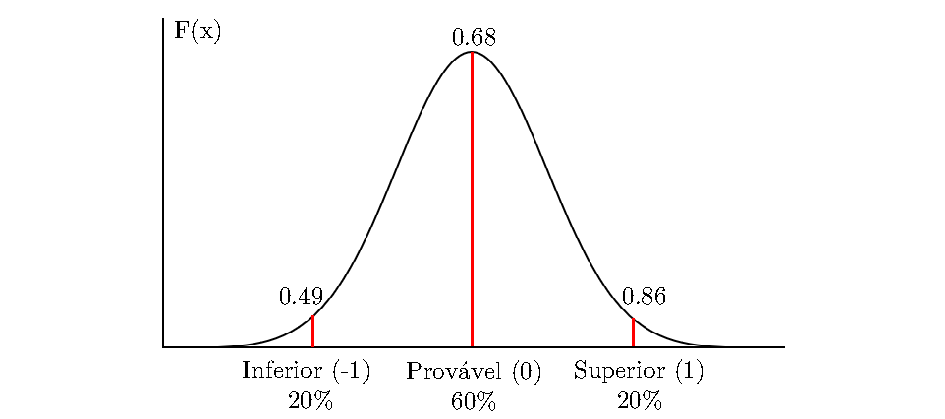
\includegraphics{Figuras/discretizacao.pdf}  
    \caption{Função de distribuição de probabilidade da variável aleatória Forma dos cascalhos de perfuração}  
    \legend{Fonte: o autor.}
    \label{fig:discretizacao}  
\end{figure}

A Figura \ref{fig:discretizacao} ilustra a distribuição de tipo normal aplicada à variável "Forma dos cascalhos". Cabe ressaltar que a distribuição normal atribuida a esta variável aleatória não apresentou valores negativos. Neste exemplo, podemos observar o processo de discretização da variável aleatória em três níveis distintos (-1= 0.49; 0= 0.68; 1= 0.86), que desempenha um papel fundamental para possibilitar as etapas de Planejamento de experimentos e Análise de risco, proporcionando uma melhor compreensão do comportamento das variáveis e seus efeitos no estudo em questão. Essa abordagem de discretização foi aplicada de forma semelhante às outras variáveis, considerando as respectivas funções de densidade de probabilidade, conforme descrito na Tabela \ref{tab:atributos}. Ao seguir essa lógica, é possível realizar análises mais detalhadas e precisas, 


\begin{table}[h]
\caption{Distribuição, níveis e probabilidades das variáveis aleatórias consideradas nesta dissertação.} 
    \begin{tabularx}{\textwidth}{llcc}
     \toprule
Atributo&Tipo de distribuição&Níveis&Probabilidades\\
  
    \midrule
    \multirow Tamanho do cascalho & Contínua (triangular)& 0 = 0.55 mm&0.60\\
    && -1 = 0.24 mm&0.20 \\
    && 1 = 0.86 mm &0.20\\
    
   \midrule
    \multirow Forma do cascalho & Contínua (normal)& 0 = 0.49 shpt&0.60\\
    && -1 = 0.68 shpt&0.20 \\
    && 1 = 0.86 shpt &0.20\\

    \midrule
    \multirow Densidade do cascalho & Contínua (gamma)& 0 = 2650 kg/m³&0.60\\
    && -1 = 2350 kg/m³&0.20 \\
    && 1 = 2950 kg/m³ &0.20\\

     \midrule
    \multirow Densidade do fluido & Contínua (lognormal)& 0 = 1375 kg/m³&0.60\\
    && -1 = 1250 kg/m³&0.20 \\
    && 1 = 1500 kg/m³ &0.20\\

    \midrule
    \multirow Viscosidade do Fluido & Contínua (triangular)& 0 = 25 cP&0.60\\
    && -1 = 15 cP&0.20 \\
    && 1 = 35 cP &0.20\\

 \midrule
    \multirow Velocidade de escoamento & Contínua(triangular)& 0 = 8.87 m/s&0.60\\
    && -1 = 9.50 m/s&0.20 \\
    && 1 = 10.13 m/s &0.20\\

    \midrule
    \multirow Vazão mássica & Contínua(triangular)& 0 = 0.13 kg/s&0.60\\
    && -1 = 0.20 kg/s&0.20 \\
    && 1 = 0.27 kg/s&0.20\\
    
    \bottomrule   
    
    \end{tabularx}
    \label{tab:atributos}
 \subcaption{Forma do cascalho (shpt) = relação entre a área da partícula e seu perímetro.}
\legend {Fonte: o autor.}
\end{table*}
\end{table}


\section{Modelo de Simulação Fluidodinâmica computacional}

Para obter quantitativamente o valor da taxa erosiva nos diversos cenários aplicados a este estudo, para emprego da análise de risco, foi necessário a elaboração de um modelo de simulação numérica por fluidodinâmica computacional, o qual apresenta diversas etapas de aplicação. A metodologia de simulação fluidodinâmica segue as etapas descritas anteriormente no capítulo \ref{Simulação Fluidodinâmica computacional (CFD)}, que necessita do desenho da geometria da curva analisada, a criação da malha computacional, a escolha dos modelos e equações para a resolução numérica de fluxo de fluido e partículas, a análise de convergência física e de resíduos e a obtenção da taxa erosiva para os diversos cenários de simulação empregados para análise de risco de falha.

\vspace{1cm}


As Simulações CFD para análise de erosão em curvas de tubulação envolvem a modelagem de múltiplos fenômenos físicos, incluindo o escoamento de fluido, o transporte de partículas sólidas, a interação partícula-parede e a erosão da parede. Portanto, a simulação pode ser computacionalmente intensiva e pode levar de algumas horas a vários dias para ser concluída, dependendo da resolução da malha (mesh), da complexidade da geometria, da precisão requerida, do poder de computação disponível e do tipo de modelagem (estacionária ou dinâmica) para execução das simulações. 

A Modelagem estacionária é baseada na suposição de que a taxa de erosão é constante em uma determinada área ao longo do tempo. Esse tipo de modelagem é mais simples e requer menos dados do que a modelagem dinâmica, mas não leva em conta as variações temporais na taxa de erosão. 

A Modelagem dinâmica leva em conta as variações temporais na taxa de erosão, permitindo uma análise mais detalhada dos processos de erosão. Esse tipo de modelagem é mais complexo e requer mais dados do que a modelagem estacionária, mas é mais preciso na estimativa da taxa de erosão ao longo do tempo. 

Por se tratar de um estudo que demanda muitos cenários de simulação para elaboração dos metamodelos e das curvas de risco, a modelagem dinâmica demandaria demasiado esforço computacional e se tornaria impraticável diante dos recursos computacionais disponíveis. Deste modo este trabalho realizou simulações CFD estacionárias para obtenção dos desgastes erosivos na tubulação curva nos diversos cenários probabilísticos estudados.

A geração da geometria é uma das fases mais importantes para a concepção da simulação Fluidodinâmica computacional, pois deve caracterizar toda a região onde ocorre o escoamento e o desgaste erosivo decorrente do impacto de partículas oriundas da perfuração de camadas rochosas. Por se tratar de um estudo envolvendo linhas hidráulicas de sistemas \textit{offshore}, este equipamento foi reproduzido com os diâmetros e geometria originais em ambiente computacional, a fim de reproduzir suas características físicas. A Figura \ref{fig:cfdgeometria} demonstra o desenho em CAD (\textit{Computer aided design}) da curva de 90 graus frequentemente utilizada nas operações de perfuração de poços de acordo com a norma de práticas recomendadas para projetos e instalação de sistemas de tubulação em plataformas de petróleo offshore \cite{api14e}. 

\begin{figure}[H] 
    \centering  
    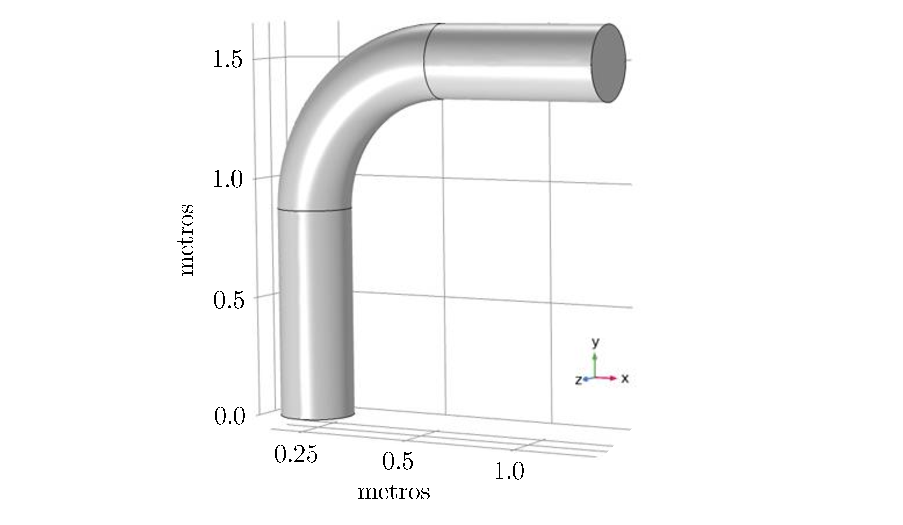
\includegraphics[width=1\textwidth]{Figuras/cfdegeometria.pdf}
    \caption{Desenho em CAD da geometria da curva de 90 graus.}  
    \legend{Fonte: o autor.}
    \label{fig:cfdgeometria}  
\end{figure}

\vspace{0.2cm}

A geometria utilizada foi de um tubo curvado de 90 graus raio
curto, de diâmetro nominal de 3 polegadas \textit{schedule} XXS. O material da curva é composto por Aço Carbono (ASTM-A 234 Gr. WPB), conforme sugerido por norma para operações em plataformas offshore \cite{api14e}. Cabe ressaltar que o material da curva influencia diretamente na magnitude do desgaste erosivo, porém a influência da geometria da curva e alteração de material não é objeto de estudo deste trabalho. Portanto, a curva de 90º de raio curto será a única avaliada para a composição da análise de risco, por ser utilizada com frequência em sistemas hidráulicos de perfuração e sugerida pela norma \cite{api14e}.

A geração da malha é uma etapa importante em simulações de CFD, com influência
direta no sucesso das simulações, entretando o número ideal de elementos de malha deve ser obtido para diminuição do tempo computacional requerido para as simulações. Para tanto, foi realizado um teste de independência da malha  para descobrir o tamanho ideal do número de elementos, com objetivo de gerar simulações de fluxo confiáveis e com custo computacional adequado (Figura \ref{fig:refmalha}).

\begin{figure}[H] 
    \centering  
    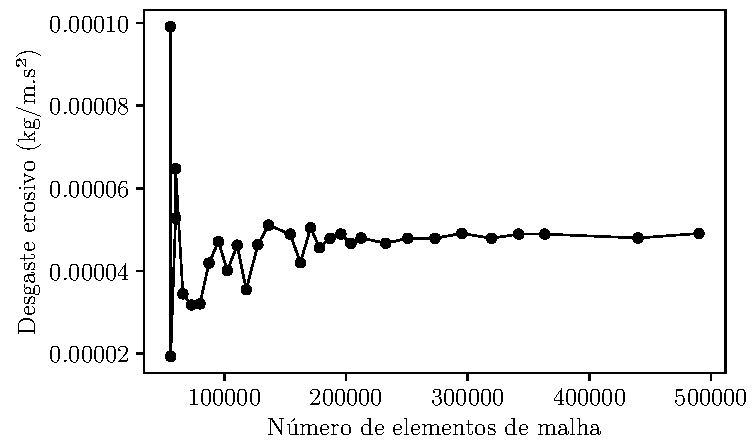
\includegraphics[textwidth=0.85\textwidth]{Figuras/testedemalha.pdf}  
    \caption{Teste de indpendência de malha para simulação fluidodinâmica computacional.}  
    \legend{Fonte: o autor.}
    \label{fig:refmalha}  
\end{figure}

É possível observar que a partir de 200.000 elementos, a solução é independente da malha. O incremento no número de elementos não influencia na resposta do dano erosivo para o modelo de simulação, ou seja, a taxa erosiva não apresentou mudanças maiores que 1\%. A Figura \ref{fig:malhaerosao} demonstra a malha computacional gerada, que compreende o total de 200.000 elementos. A malha contém elementos hexaédricos com refinamento na região de interesse para minimizar a ocorrência de elementos distorcidos \cite{zhang}.

\begin{figure}[H] 
    \centering  
    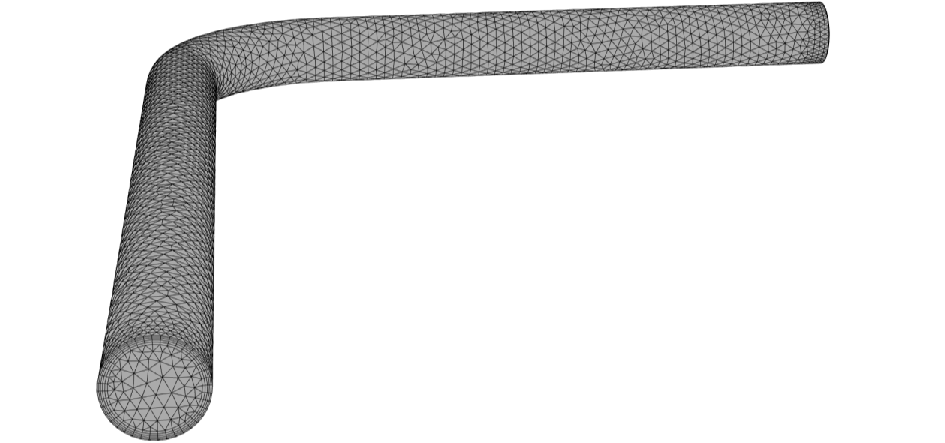
\includegraphics[textwidth=0.33\textwidth]{Figuras/MALHA.pdf}  
    \caption{Malha computacional da curva de 90 graus.}  
    \legend{Fonte: o autor.}
    \label{fig:malhaerosao}  
\end{figure}

Após criação da malha, nomeou-se as condições de contorno da curva de aço carbono (Figura \ref{fig:condcontorno}). As condições de contorno definem as regiões de entrada e saída do fluido e dos cascalhos na tubulação, e a delimitação do sistema físico através da definição da região de parede da tubulação.

\begin{figure}[H] 
    \centering  
    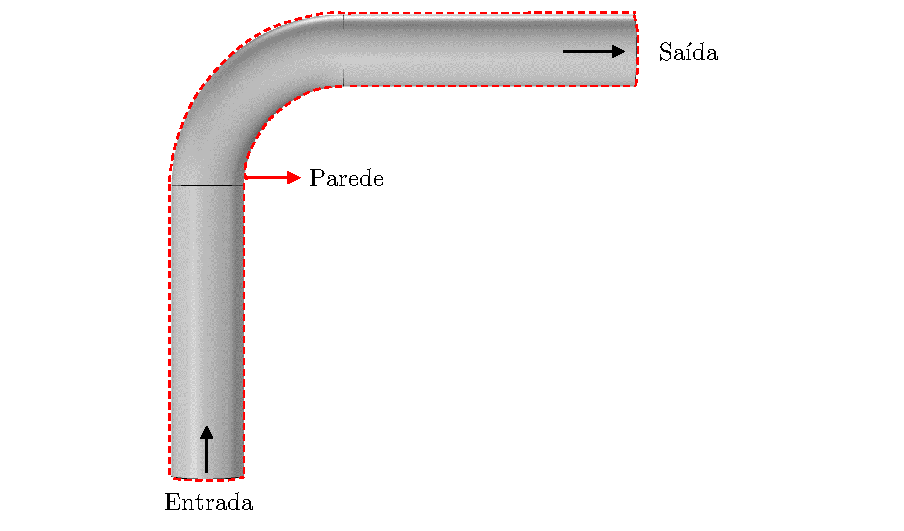
\includegraphics{Figuras/contornoregiao.pdf}  
    \caption{Condições de contorno da curva de aço carbono de 90 graus.}  
    \legend{Fonte: o autor.}
    \label{fig:condcontorno}  
\end{figure}

Para as simulações realizadas neste estudo, foi definido o regime de escoamento como permanente, o qual não considera a variação do tempo como influência direta nos atributos de entrada. A turbulência foi modelada utilizando  as equações de k-e, este modelo foi utilizado nas simulações numéricas validadas por ensaios experimentais de erosão no estudo de \citeonline{liuuh}. O modelo k-e reproduz um regime turbulento e multifásico, onde "k" é a energia cinética da turbulência "e" 
 é a dissipação turbulenta. Para a resolução numérica de escoamentos de fluidos isotérmicos e incompressíveis, foi utilizado as equações de Navier Stokes com médias em Reynolds (RANS).

Para reproduzir um fluxo multifásico envolvendo o transporte de cascalhos e  de fluido e particulado (cascalhos), foi utilizado o modelo Euleriano-Lagrangeano de fase discreta DPM (Discrete Phase Model). A abordagem do método Lagrangeano permite rastrear o trajeto das partícula no sistema computacional, o que propicia estimar qualitativamente as regiões de impacto de partículas e quantitativamente a magnitude do desgaste erosivo.

Tendo em vista que as equações governantes são interdependentes e não lineares, o processo de solução é caracterizado por iterações até que as equações de continuidade, quantidade de movimento e de turbulência atinjam a solução convergindo para valores residuais baixos. Deste modo, a convergência dos modelos será analisada verificando os resíduos das equações governantes do modelo. Embora haja baixos valores residuais e um comportamento de convergência das equações governantes, é possível que a solução física de escoamento não convirja. Desse modo, como alternativa complementar para análise do modelo, será monitorado a convergência física do parâmetro de velocidade de escoamento na saída do fluido do sistema.


Cabe ressaltar que a faixa de variação do estudo considerou uma proporção volumétrica menor que 10\% de cascalhos em todos os cenários obtidos, ou seja, a quantidade de partículas presentes não extrapolaram o limite definido pelo método matemático utilizado. Essa restrição foi estabelecida para garantir que a fase discreta, representada pelas partículas de cascalho, não influenciasse significativamente o fluxo da fase contínua. Dessa forma, foi viável utilizar o modelo de modelagem da fase discreta (DPM) ou Discrete Phase Model nas Simulações Fluidodinâmicas para todo o estudo constituído. O equacionamento da trajetória das partículas lagrangeanas foi calculado separadamente da fase contínua, permitindo uma análise precisa e independente do comportamento das partículas de cascalho no sistema.



\section{Análise de Sensibilidade}

A análise de sensibilidade é uma abordagem que visa avaliar a influência dos atributos ou variáveis de um sistema na resposta ou resultado desejado. Ela permite identificar quais fatores têm maior impacto na função-objetivo e entender a relação entre as variáveis e a resposta. O método utilizado para realizar a análise de sensibilidade foi o gráfico de tornado, que consistiu em variar os atributos em níveis inferiores e superiores, mantendo os demais atributos fixos, e observar o impacto percentual dessas variações na resposta do desgaste erosivo. O gráfico de tornado exibiu os valores de sensibilidade de cada atributo, representados por barras, onde a altura das barras indica a magnitude do impacto na resposta. Essas barras são ordenadas em ordem decrescente, permitindo identificar quais atributos têm maior influência na resposta. A metodologia de triagem por Plackett Burman, descrita no capítulo \ref{sec:Planejamentoestatistico} foi com os resultados de Análise de sensibilidade para definição dos atributos críticos.



\section{Planejamento estatístico}
\label{sec:Planejamentoestatistico}

Neste trabalho, o planejamento estatístico foi utilizado em duas etapas. Inicialmente, aplicado para a seleção dos atributos críticos, ou seja, aqueles que apresentam maior influência na função-objetivo analisada. A segunda etapa objetivou a obtenção da Superfície de resposta, com a finalidade de gerar um metamodelo de regressão para substituição do simulador numérico CFD. A Figura \ref{fig:planestatistico} ilustra todo o procedimento utilizado nesta etapa. 


\begin{figure}[H] 
    \centering  
    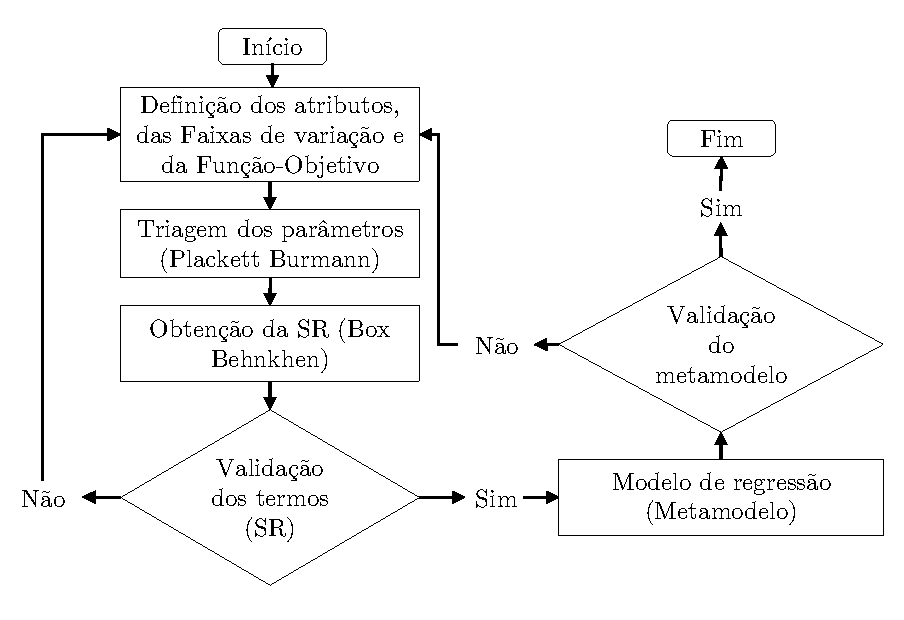
\includegraphics{Figuras/suprespostametodologia.pdf}  
    \caption{Metodologia de Planejamento estatístico.}  
    \legend{Fonte: Adaptado de \citeonline{lemma}}
}
    \label{fig:planestatistico}  
\end{figure}


Na etapa inicial, foi necessário definir os atributos incertos, estabelecer sua faixa de valores e determinar a distribuição de probabilidade das variáveis que poderiam influenciar as previsões da taxa de erosão, de acordo com o estudo bibliográfico. Nessa etapa, os atributos foram padronizados em três níveis incertos, conforme descrito na etapa de discretização das variáveis aleatórias em níveis de probabilidades (capítulo \ref{cap:Variáveis aleatórias e distribuições de probabilidades}).

 Neste trabalho, para a etapa de triagem dos atributos, as simulações numéricas foram realizadas conforme um planejamento experimental fatorial fracionado do tipo Plackett–Burman, com objetivo de comparar os resultados com a Análise de sensibilidade. Esta aplicação é adequada para realizar uma análise superficial na fase inicial de estudo, uma vez que requer poucos experimentos. Foram estudadas estatisticamente a influência de 7 atributos na taxa erosiva:  Tamanho do cascalho, Forma do cascalho, Densidade do cascalho, Densidade do fluido de perfuração, Viscosidade do fluido de perfuração, Velocidade de escoamento e Vazão mássica. A Tabela \ref{tab:box4} apresenta a matriz do planejamento utilizado nesta etapa e os respectivos valores das variáveis aleatórias estudadas.

\begin{table}[H] 
\caption{Matriz do planejamento Plackett Burmann para 7 variáveis de entrada.}
\begin{tabular*}{\textwidth}{@{\extracolsep{\stretch{1}}}*{8}{c}@{}}
\toprule
   Simulação &VM&	DC	&TAM	&VEL&	FM&	DF	&VISC\\
  \midrule
01 & 0.13 &	2350 &	0.24	& 8.87   &	0.49 &	1250 &	15 	\\
02 & 0.13 &	2950 &	0.86	& 8.87  &	0.87 &	1250 &	15 	\\
03 & 0.27 &	2350 &	0.24	& 8.87  &	0.87 &	1500 &	35   \\
04 & 0.13 &	2950&	0.24	& 8.87   &	0.49 &	1500 &	35    \\
05 & 0.13 &	2950 &	0.86	& 10.13  &	0.49 &	1500 &	35     \\
06 & 0.27 &	2950 &	0.24	& 10.13	 &  0.87 &	1250 &	35     \\
07 & 0.27 &	2350 &	0.86	& 10.13	 &  0.49 &	1500 &	15 	\\
08 & 0.13 &	2350 &	0.86	& 10.13 &  0.87 &	1250 &	35 	\\
09 & 0.13 &	2350 &	0.24	& 10.13	 &  0.87 &	1500&	15 	\\
10 & 0.27 &	2350 &	0.86	& 8.87	 &  0.49 &	1250&	35 	\\
11 & 0.27 &	2950 &	0.86	& 8.87	 &  0.87 &	1500&	15 	\\
12 & 0.27 &	2950 &	0.24    & 10.13	 &  0.49 &	1250 &	15	\\

\bottomrule   
\end{tabular*}
\label{tab:box4}
\subcaption{VM: Vazão massica(kg/s); VISC: Viscosidade do fluido de perfuração(cP); TAM: Tamanho(mm); VEL: Velocidade de escoamento(m/s).}
\legend {Fonte: o autor.}
\label {tab:placket7var}
\end{table}

Na segunda etapa, o objetivo foi identificar os parâmetros que possuem um impacto significativo na função objetivo. Isso foi feito por meio da análise de variância (ANOVA), a fim de determinar a melhor maneira de conduzir estudos adicionais, como a construção da superfície de resposta e a análise de risco, com o menor custo computacional possível.

Após a realização da análise de variância do planejamento de Plackett-Burman proposto e a análise de sensibilidade, foram selecionadas as variáveis mais significativas em relação ao desgaste erosivo. Essas variáveis foram utilizadas na elaboração da matriz de experimentos de Box-Behnken, que é uma técnica de planejamento experimental que permite explorar de forma eficiente a região de interesse e obter informações sobre as interações entre as variáveis.

Para a obtenção da Superfície de resposta (SR), foi realizada a combinação dos termos definidos em uma matriz de ensaio experimental definida pelo planejamento estatístico de Box Benhkhen. O número total de simulações realizadas para a matriz de Box Behkehn é \textit{N = 2 * k * (k − 1) + Co}, em que \textit{k} é o número de atributos e \textit{Co} é o número de pontos centrais. A Tabela \ref{tab:box5555} apresenta a matriz codificada do planejamento utilizado nesta etapa e os respectivos valores das variáveis. As variáveis presentes nos ensaios computacionais, foram definidas na etapa de triagem de atributos por análise de sensibilidade e significância estatística dos termos por Plackett Burmann, que seráão detalhadas nos resultados do capítulo \ref{sec:Seleçãodosatributoscríticos} .

\begin{table}[H]
\caption{Matriz do planejamento Box Benhkhen para 4 variáveis de entrada.}
\begin{tabular*}{\textwidth}{@{\extracolsep{\stretch{1}}}*{5}{c}@{}}
 \toprule
   Simulação &VM	&VISC	&TAM	&VEL	\\
  \midrule

1         & 0.13 & 15   & 0.55 & 9.50  \\
2         & 0.27 & 15   & 0.55 & 9.50  \\
3         & 0.13 & 35   & 0.55 & 9.50  \\
4                                 & 0.27                         & 35   & 0.55 & 9.50  \\
5                                 & 0.20                         & 25   & 0.24 & 8.87  \\
6                                 & 0.20                         & 25   & 0.86 & 8.87  \\
7                                 & 0.20                         & 25   & 0.24 & 10.13 \\
8                                 & 0.20                         & 25   & 0.86 & 10.13 \\
9                                 & 0.13                         & 25   & 0.55 & 8.87  \\
10                                & 0.27                         & 25   & 0.55 & 8.87  \\
11                                & 0.13                         & 25   & 0.55 & 10.13 \\
12                                & 0.27                         & 25   & 0.55 & 10.13 \\
13                                & 0.20                         & 15   & 0.24 & 9.50  \\
14                                & 0.20                         & 35   & 0.24 & 9.50  \\
15                                & 0.20                         & 15   & 0.86 & 9.50  \\
16                                & 0.20                         & 35   & 0.86 & 9.50  \\
17                                & 0.13                         & 25   & 0.24 & 9.50  \\
18                                & 0.27                         & 25   & 0.24 & 9.50  \\
19                                & 0.13                         & 25   & 0.86 & 9.50  \\
20                                & 0.27                         & 25   & 0.86 & 9.50  \\
21                                & 0.20                         & 15   & 0.55 & 8.87  \\
22                                & 0.20                         & 35   & 0.55 & 8.87  \\
23                                & 0.20                         & 15   & 0.55 & 10.13 \\
24                                & 0.20                         & 35   & 0.55 & 10.13 \\
25                                & 0.20                         & 25   & 0.55 & 9.5  \\

\bottomrule 
\end{tabular*}
\label{tab:box5555}
\subcaption{VM: Vazão massica(kg/s); VISC: Viscosidade do fluido de perfuração(cP); TAM: Tamanho(mm); VEL: Velocidade de escoamento(m/s).}
\legend {Fonte: o autor.}
\end{table}



A análise estatística do planejamento de Box Benhkhen foi realizada através da aplicação da Análise de Variância (ANOVA) aos termos da Superfície de Resposta, avaliando o p-valor e Teste F dos termos lineares, de interação e quadráticos. Foi estimada a precisão adequada do modelo para verificar a relação entre sinal-ruído, comparando o range de valores previstos pelo modelo nos pontos de ensaios da matriz de experimentos com o erro médio de previsão. 

Com a estrutura de dados adquirida e validada estatisticamente, foi obtida a equação matemática com os termos significativos que descreve a resposta da superfície. Em seguida, os valores simulados de desgaste erosivo utilizados para construir a resposta da superfície foram comparados com os valores obtidos de desgaste erosivo pela equação de regressão do modelo, a fim de realizar o teste de consistência, ou seja, verificar se o modelo está prevendo adequadamente os dados de simulação numérica. A validação cruzada foi realizada comparando os valores obtidos pela simulação com os valores previstos pelo modelo de regressão. Os coeficientes de determinação R², R² ajustado e R² predito foram utilizados para avaliar a qualidade do modelo. Se os termos do modelo não forem estatisticamente validados ou se a validação cruzada não apresentar um bom coeficiente de determinação, as etapas da metodologia devem ser refeitas. Ao passo que o metamodelo de regressão passar pela verificação de validação estatística e que não apresente caracteristicas consideravelmente divergentes da simulação numérica CFD, ele pode ser aplicado para prever novos cenários de erosão. Neste trabalho, o metamodelo foi utilizado para gerar curvas de risco para a função-objetivo de erosão de \citeonline{oka} nos processos de análise que envolvem muitos cenários de simulação (Monte Carlo e Árvore de derivação). 

A validação das respostas dos modelo gerados pelos planejamentos de experimentos de Plackett-Burmann e Box Benhkhen requer a aplicação de testes estatísticos recomendados por \cite{montgomery}. Esses testes são essenciais para avaliar a adequação do modelo aos dados. Uma das etapas dessa validação envolve a análise da normalidade dos resíduos do modelo. Com este objetivo, foi utilizado o gráfico de probabilidade normal com objetivo comparar a função de distribuição acumulada empírica (ECDF) dos resíduos com a distribuição esperada para resíduos com comportamento normal. Também foi aplicado o teste de hipóteses de Kolmogorov-Smirnoff que consiste em uma técnica estatística não paramétrica que é usada para verificar se existem evidências de normalidade dos resíduos. Além disso, foi de suma importância verificar a constância da variância dos resíduos, ou seja, se eles apresentavam evidências de homocedasticidade. A suposição de homocedasticidade era fundamental para a análise de regressão do modelo ajustado. Caso os resíduos demonstrassem uma dispersão constante em relação aos valores preditos, validava-se a suposição de homocedasticidade.


\section{Análise de Risco por Árvore de Derivação}

A composição da Árvore de Derivação foi realizada a partir dos resultados da análise de sensibilidade e de Plackett Burmann, ou seja, somente os atributos críticos (z) e seus respectivos níveis de incerteza (y) foram utilizados para combinação para obtenção da curva de risco. O número de ramificações, ou seja, a quantidade de combinações presentes na Árvore de derivação é representada por $y^z$ = modelos de simulação. Deste modo, a partir da definição dos atributos críticos foram gerados 81 cenários de simulação para composição da Árvore de derivação. Após simulação fludidinâmica dos cenários determinados, os dados foram tratados estatisticamente para obtenção da curva de risco de falha por erosão.


\section{Análise de risco por Monte Carlo}


Uma etapa de análise de risco realizada neste trabalho, é o emprego da técnica de
Monte Carlo para a combinação dos atributos críticos e obtenção da curva de risco de falha por erosão. A Figura \ref{fig:montecarloflux} demonstra as etapas realizadas para a composição dos cenários de simulação de Monte Carlo.

\begin{figure}[H] 
    \centering  
    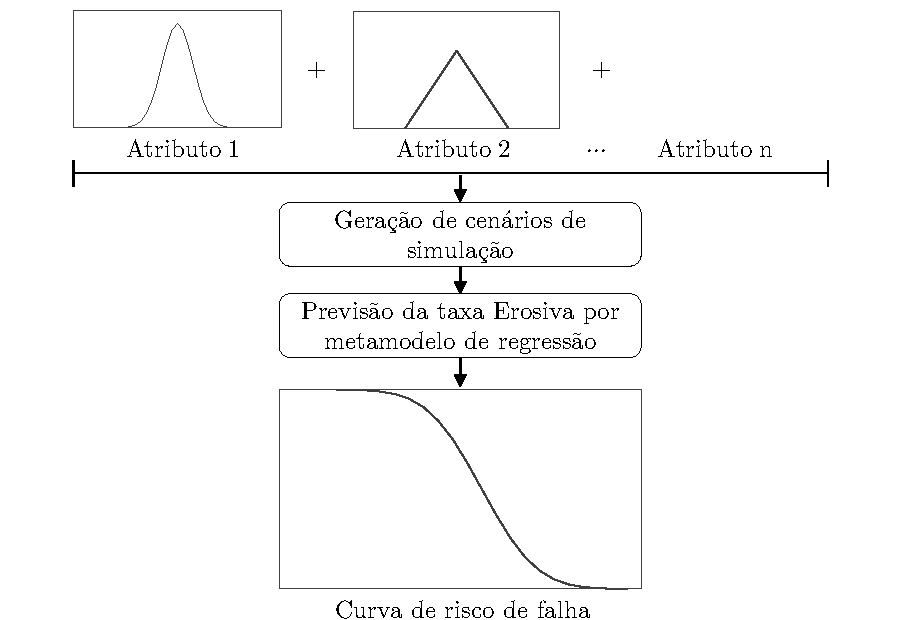
\includegraphics{Figuras/metodologiaMC.pdf}  
    \caption{Metodologia de Monte Carlo para Análise de risco de falha por erosão.}  
    \legend{Fonte: o autor.}
    \label{fig:montecarloflux}  
\end{figure}

Na primeira etapa, foram realizadas amostragens aleatórias nos atributos que exercem influência sobre a taxa erosiva de Oka, determinados no planejamento estatístico de Plackett Burmann. Os valores foram amostrados de acordo com a distribuição de probabilidade de cada variável. Assim, os atributos foram combinados para gerar um número elevado de cenários e produzir uma estimativa consistente da função de distribuição de probabilidade para a resposta de erosão do modelo de Oka. Para estimar o número de cenários ideal para o método de Monte Carlo, foi utilizado o cálculo do coeficiente de variação (CoV), que é um indicador de flutuação em torno da média de uma variável aleatória. O Cov é um parâmetro adimensional, dado por:

\begin{equation}
    CoV (\%) =  \frac{\sigma X}{\mu X}
\end{equation}

Na qual:

$\sigma$X= Média amostral;

$\mu$X= Desvio padrão amostral.

\vspace{0.3cm}

O número de cenários ideal para os sorteios de Monte Carlo foi definido a partir da estabilização do coeficiente de variação (Cov), obtido pelos diferentes cenários realizados pelo método de Monte Carlo. Devido ao elevado número de cenários, para previsão da resposta de erosão de Oka, foi utilizado o metamodelo de regressão gerado pelo planejamento de Superfície de resposta. A partir das respostas dos cenários, foi possível obter as curvas de risco. Nessa etapa, foram plotadas curvas geradas com diferentes números de sorteios, a fim de avaliar a influência da quantidade de cenários nas respostas do método de Monte Carlo e comparar com a curva de risco gerada pelo método de Árvore de derivação.






